\Needspace{6.5in}

\begin{prob}

    A modification of the \texttt{dfs} function from lecture is shown below.
    It is the same as the original \texttt{dfs} function, except that it has
    an added \texttt{print} statement.

    \begin{minted}[autogobble]{python}
        def dfs(graph, u, status=None):
            """Start a DFS at `u`."""
            # initialize status if it was not passed
            if status is None:
                status = {node: 'undiscovered' for node in graph.nodes}

            status[u] = 'pending'
            for v in graph.neighbors(u):
                if status[v] == 'undiscovered':
                    print("Hello!")
                    dfs(graph, v, status)
            status[u] = 'visited'
    \end{minted}

    Consider running this algorithm on the following graph, starting at node $a$:

    \begin{center} 
    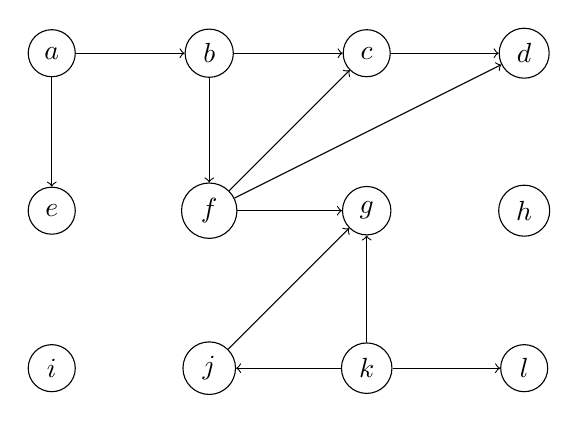
\begin{tikzpicture}
        \tikzset{every node/.style = {shape=circle, draw, minimum size=17pt}}

        \node (a) at (0, 0) {$a$};
        \node (b) at (2, 0) {$b$};
        \node (c) at (4, 0) {$c$};
        \node (d) at (6, 0) {$d$};

        \node (e) at (0, -2) {$e$};
        \node (f) at (2, -2) {$f$};
        \node (g) at (4, -2) {$g$};
        \node (h) at (6, -2) {$h$};

        \node (i) at (0, -4) {$i$};
        \node (j) at (2, -4) {$j$};
        \node (k) at (4, -4) {$k$};
        \node (l) at (6, -4) {$l$};

        \draw (a) edge[->] (b);
        \draw (b) edge[->] (c);
        \draw (c) edge[->] (d);

        \draw (a) edge[->] (e);
        \draw (b) edge[->] (f);

        \draw (k) edge[->] (l);

        \draw (j) edge[->] (g);
        \draw (k) edge[->] (g);
        \draw (k) edge[->] (j);

        \draw (f) edge[->] (g);
        \draw (f) edge[->] (c);
        \draw (f) edge[->] (d);

    \end{tikzpicture}
    \end{center}

    How many times will \python{"Hello!"} be printed? Note that this is not a full DFS, and
    that not all nodes are reachable from $a$.

    \inlineresponsebox[.75in]{6}

\end{prob}
